%! Author = fusel
%! Date = 24.07.21

% Preamble
\documentclass[final]{fhnwreport}
% Packages
\usepackage{amsmath}
\usepackage{lipsum}
\usepackage[german]{babel}
\usepackage[style=ieee,urldate=comp,backend=biber]{biblatex}
\usepackage{listings}
\usepackage{xcolor}
\usepackage{dirtree}
\usepackage{textcomp}
\usepackage{tabularx}
\usepackage{blindtext}
\usepackage{import}
\addbibresource{main.bib}

% Custom JS Listing support
\definecolor{mygreen}{rgb}{0,0.6,0}
\definecolor{mygray}{rgb}{0.5,0.5,0.5}
\definecolor{mymauve}{rgb}{0.58,0,0.82}
%Customize a bit the look
\lstset{ %
    backgroundcolor=\color{white}, % choose the background color; you must add \usepackage{color} or \usepackage{xcolor}
    basicstyle=\footnotesize, % the size of the fonts that are used for the code
    breakatwhitespace=false, % sets if automatic breaks should only happen at whitespace
    breaklines=true, % sets automatic line breaking
    captionpos=b, % sets the caption-position to bottom
    commentstyle=\color{mygreen}, % comment style
    deletekeywords={...}, % if you want to delete keywords from the given language
    escapeinside={\%*}{*)}, % if you want to add LaTeX within your code
    extendedchars=true, % lets you use non-ASCII characters; for 8-bits encodings only, does not work with UTF-8
    frame=single, % adds a frame around the code
    keepspaces=true, % keeps spaces in text, useful for keeping indentation of code (possibly needs columns=flexible)
    keywordstyle=\color{blue}, % keyword style
% language=Octave, % the language of the code
    morekeywords={*,...}, % if you want to add more keywords to the set
    numbers=left, % where to put the line-numbers; possible values are (none, left, right)
    numbersep=5pt, % how far the line-numbers are from the code
    numberstyle=\tiny\color{mygray}, % the style that is used for the line-numbers
    rulecolor=\color{black}, % if not set, the frame-color may be changed on line-breaks within not-black text (e.g. comments (green here))
    showspaces=false, % show spaces everywhere adding particular underscores; it overrides 'showstringspaces'
    showstringspaces=false, % underline spaces within strings only
    showtabs=false, % show tabs within strings adding particular underscores
    stepnumber=1, % the step between two line-numbers. If it's 1, each line will be numbered
    stringstyle=\color{mymauve}, % string literal style
    tabsize=2, % sets default tabsize to 2 spaces
    title=\lstname % show the filename of files included with \lstinputlisting; also try caption instead of title
}
%END of listing package%

\definecolor{darkgray}{rgb}{.4,.4,.4}
\definecolor{purple}{rgb}{0.65, 0.12, 0.82}

%define Javascript language
\lstdefinelanguage{JavaScript}{
    keywords={typeof, new, true, false, catch, function, return, null, catch, switch, const, let, var, if, in, while, do, else, case, break},
    keywordstyle=\color{blue}\bfseries,
    ndkeywords={class, export, boolean, throw, implements, import, this},
    ndkeywordstyle=\color{darkgray}\bfseries,
    identifierstyle=\color{black},
    sensitive=false,
    comment=[l]{//},
    morecomment=[s]{/*}{*/},
    commentstyle=\color{purple}\ttfamily,
    stringstyle=\color{red}\ttfamily,
    morestring=[b]',
    morestring=[b]"
}

\lstset{
    language=JavaScript,
    extendedchars=true,
    basicstyle=\footnotesize\ttfamily,
    showstringspaces=false,
    showspaces=false,
    numbers=left,
    numberstyle=\footnotesize,
    numbersep=9pt,
    tabsize=2,
    breaklines=true,
    showtabs=false,
    captionpos=b
}



\title{Peer-to-Peer Kommunikation für Sprachübertragung in einem Praxisrufsystem}  %Project Title
\author{IP6 - Bachelor Thesis}                      %Document Type => Technical Report, ...

\begin{document}
    \maketitle

    \vspace*{\fill}

    \begin{center}
        \renewcommand\arraystretch{2}
        \begin{tabular}{l l}
            Studenten & Joshua Villing \\
            Fachbetreuer & Daniel Jossen\\
            Auftraggeber & Daniel Jossen\\
            Studiengang & Informatik\\
            Hochschule & Hochschule für Technik
        \end{tabular}
    \end{center}

    \clearpage


%%---ABSTRACT----------------------------------------------------------------------------
    \pagenumbering{Roman}
    \section*{Management Summary}

''Ärzte und Zahnärzte haben den Anspruch in Ihren Praxen ein Rufsystem einzusetzen.
Dieses Rufsystem ermöglicht, dass der behandelnde Arzt über einen Knopfdruck Hilfe anfordern oder Behandlungsmaterial bestellen kann.
Heute kommerziell erhältlichen Rufsysteme beruhen meistens auf proprietären Standards und veralteten Technologien.''\cite{aufgabenstellung}
Mit dem Projekt ''IP5 Cloudbasiertes Praxisrufsystem'' wurde ein modernes Rufsystem ''Praxisruf'' mit reduziertem Funktionsumfang umgesetzt.
Die Problemstellung für dieses Projekt besteht darin, das bestehende Praxisrufsystem zu erweitern und fehlende Funktionen zu ergänzen.

Das erweiterte Praxisrufsystem hat zwei Hauptfunktionen.
Es kann als Gegensprechanlage verwendet werden und bietet die Möglichkeit Benachrichtigungen in einer Praxis zu versenden.
Das Rufsystem wird von Endbenutzern über IPads bedient.
Die dazu entwickelte Applikation ermöglicht es, Sprachverbindungen zwischen zwei oder mehr Teilnehmern aufzubauen und Benachrichtigungen zu versenden.
Der Inhalt von empfangenen Benachrichtigungen kann bei entsprechender Konfiguration automatisch vorgelesen werden.
Welche Sprachverbindungen und Benachrichtigungen zur Verfügung stehen, wird von Administratoren über eine Weboberfläche konfiguriert.

Nach Projektabschluss stehen drei Optionen für das weitere Vorgehen offen:

\textbf{1. Produktiver Einsatz}

Mit den Erweiterungen, die in diesem Projekt umgesetzt wurden, erfüllt Praxisruf die Mindestanforderungen an ein modernes Praxisrufsystem.
Dementsprechend könnte das System bereits heute als produktives Rufsystem in einem Praxisumfeld eingesetzt werden.
Praxisruf allerdings noch nicht in einem produktiven Umfeld getestet.
Es muss verifiziert werden, dass das System mit der Last, die in einem produktiven Umfeld entsteht umgehen kann und den Qualitätsansprüchen von Praxismitarbeitenden entspricht.
Weiter hat das System noch Lücken in den Bereichen Benutzerfreundlichkeit und Konfigurierbarkeit.
Aufgrund dieser Einschränkung wird davon abgeraten, Praxisruf produktiv einzusetzen.

\textbf{2. Test in Pilotbetrieb}

Um Praxisruf in einem produktiven Umfeld zu testen, könnte es als Pilotprojekt in einzelnen Praxen eingesetzt werden.
In diesem Pilotprojekt könnten Rückmeldung von Praxismitarbeitenden gesammelt und Performancemetriken gemessen werden.
Aufgrund dieser Ergebnisse kann evaluiert werden, welche Erweiterungen an Praxisruf vorgenommen werden müssen.

\textbf{3. Weiterentwicklung für kommerzielle Nutzung}

Praxisruf ist heute darauf ausgelegt, in genau einer Praxis eingesetzt zu werden.
Um es als kommerziell erhältliches System anbieten zu können muss es um Mandantenfähigkeit erweitert werden.
Es muss möglich sein mehrere Systemkonfigurationen zu verwalten, wobei diese strikt voneinander getrennt bleiben.
Weiter wird empfohlen die Berechtigungsprüfung in Praxisruf zu erweitern und einen externen Identity-Provider anzubinden.

\textbf{Empfehlung}

Es wird empfohlen mit der Option zwei ''Test in Pilotbetrieb'' fortzufahren.
Durch Pilotbetrieb in einem realistischen Umfeld, kann garantiert werden, dass Praxisruf den Qualitätsanspruchen der Anwender enstpricht.
Weiter kann die Verwendung des Systems beobachtet werden und in hinsicht Performance und Benutzerfreundlichkeit wo nötig verbessert werden.
Sollte Praxisruf als kommerzielles System angeboten werden, wird zudem empfohlen die Option drei ''Weiterentwicklung für kommerzielle Nutzung'' zu verfolgen.
Die Erweiterung um Mandantenfähigkeit und Anbindung eines externen Identity-Providers sind für die kommerzielle Nutzung des Systems unerlässlich.

\clearpage



%%---TABLE OF CONTENTS-------------------------------------------------------------------
    \setcounter{tocdepth}{2}
    \tableofcontents
    \clearpage

%%---TEXT--------------------------------------------------------------------------------
    \pagenumbering{arabic}
    \section{Einleitung}

''Ärzte und Zahnärzte haben den Anspruch in Ihren Praxen ein Rufsystem einzusetzen.
Dieses Rufsystem ermöglicht, dass der behandelnde Arzt über einen Knopfdruck Hilfe anfordern oder Behandlungsmaterial bestellen kann.''\cite{aufgabenstellung}
Mit diesem Projekt wurde ein cloudbasiertes Praxisrufsystem konzipiert und umgesetzt.
Dazu wurde das im Vorgängerprojekt ''IP5 Cloudbasiertes Praxisrufsystem'' umgesetzte Praxisrufsystem erweitert.
Das erweiterte System ermöglicht es Benachrichtigungen zu versenden und Sprachverbindungen zwischen Teilnehmern aufzubauen.
Als Benutzeroberfläche dient dabei eine native iOS Applikation.
Folgende Abbildungen zeigen die Startseite der iOS Applikation (Abbildung 1.1) sowie die Ansicht während eines aktiven Gruppenanrufs (Abbildung 1.2).

\begin{figure}[h]
    \centering
    \begin{minipage}[b]{0.4\textwidth}
        \fbox{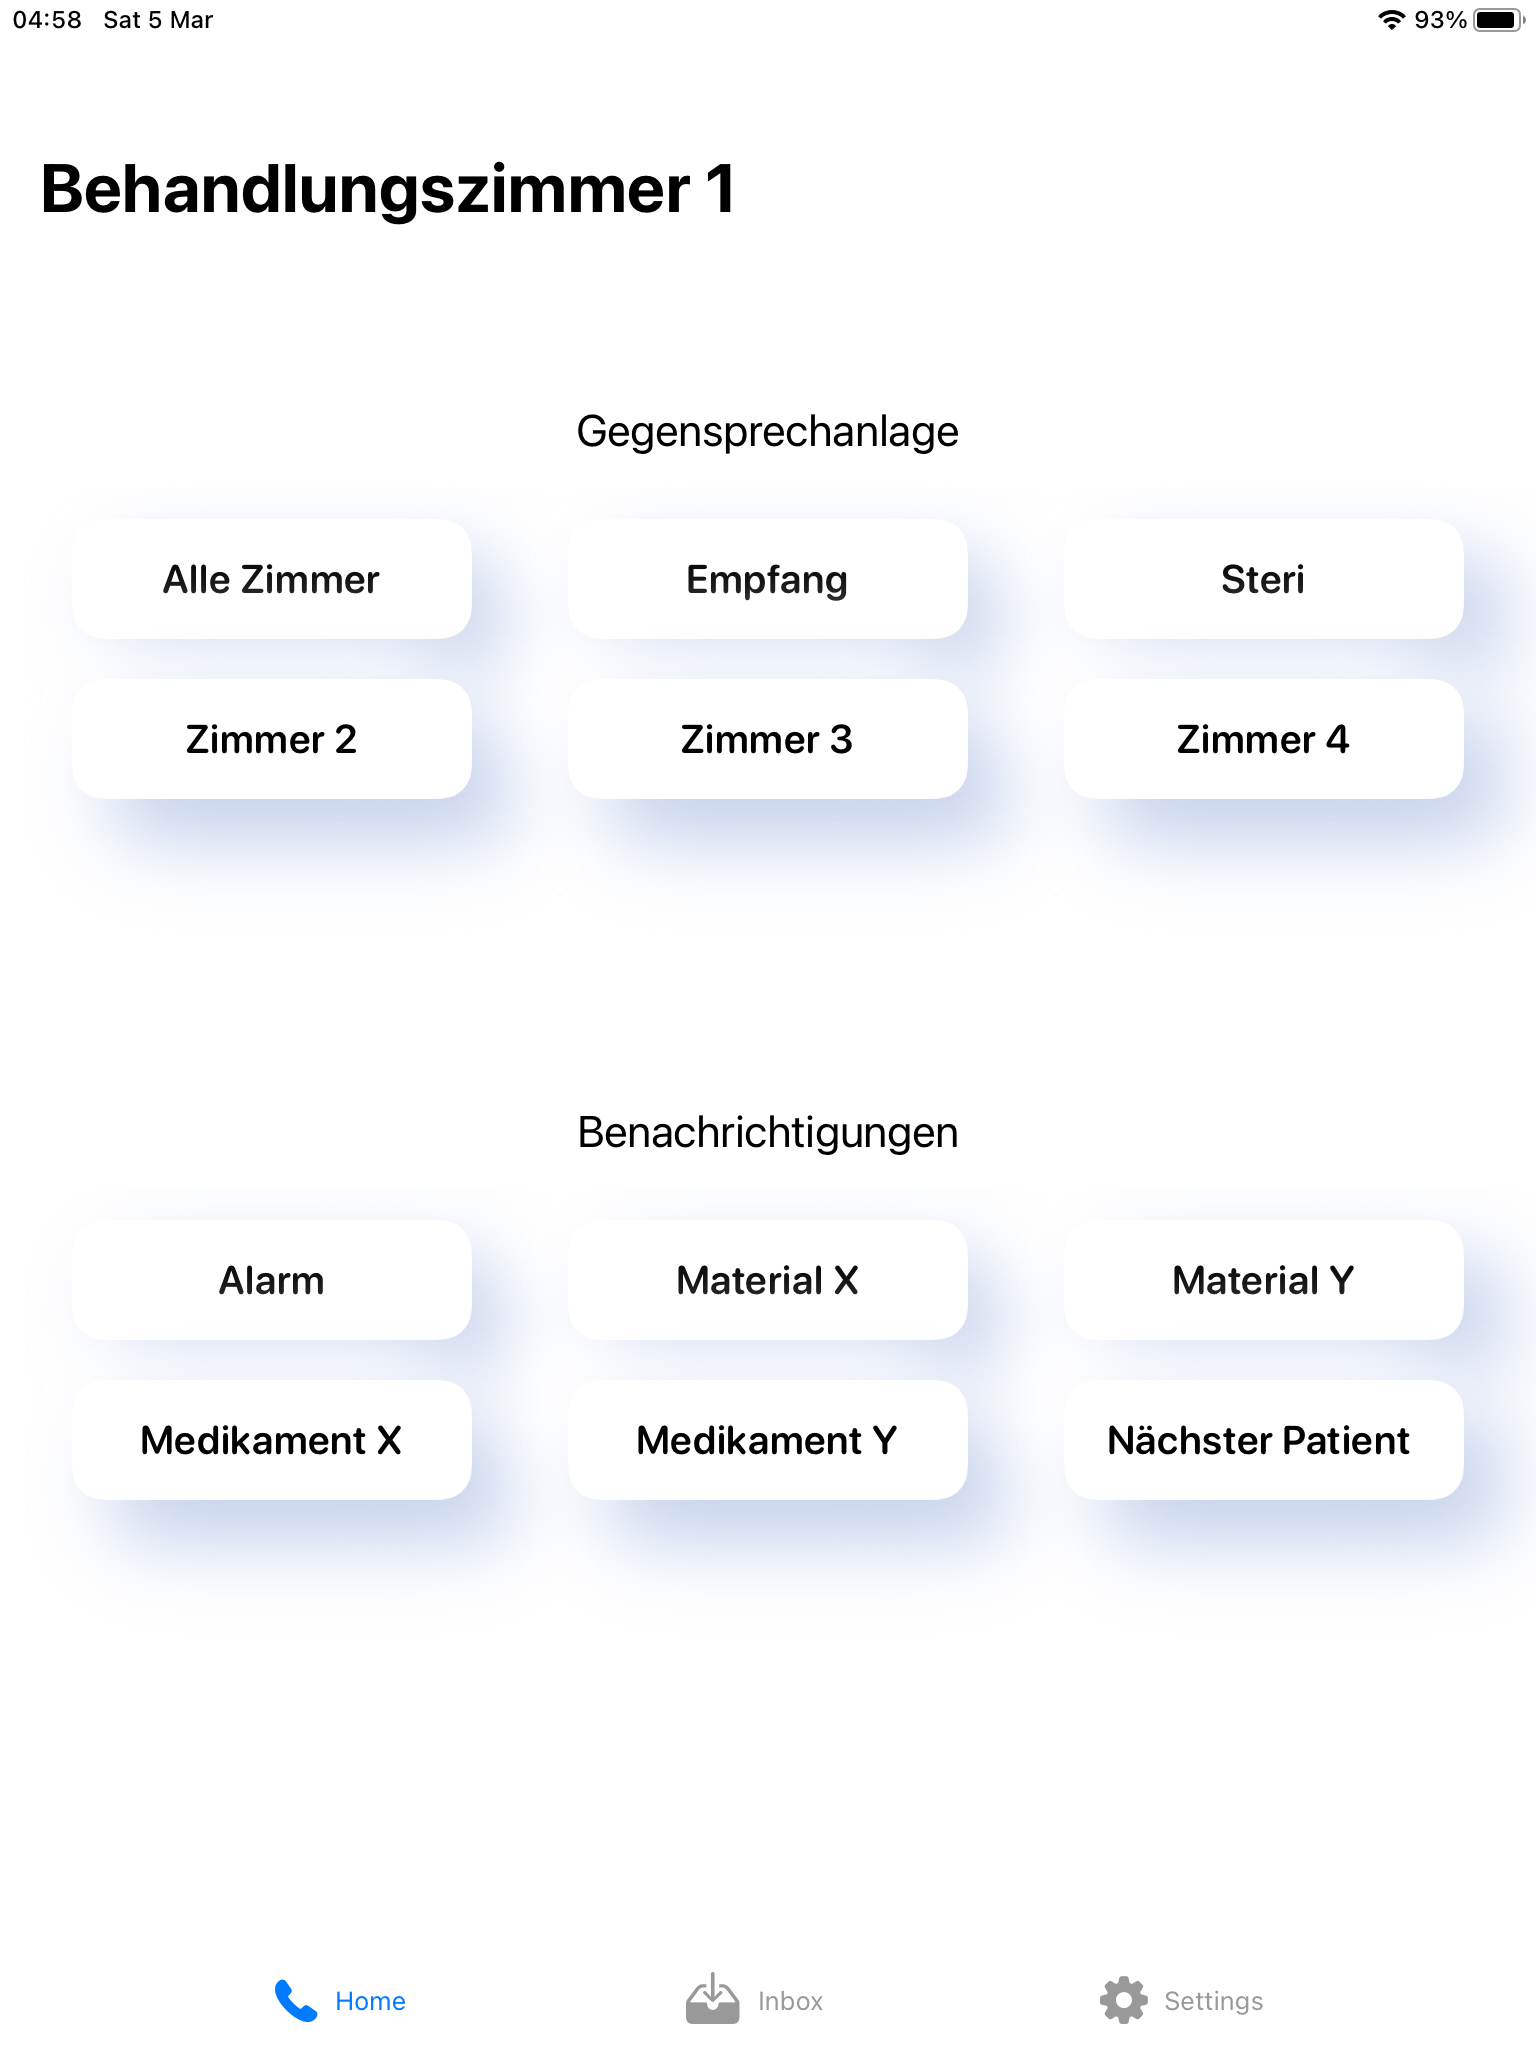
\includegraphics[width=\textwidth]{graphics/screenshots/app/home}}
        \caption{Praxisruf Startseite}
    \end{minipage}
    \hfill
    \begin{minipage}[b]{0.4\textwidth}
        \fbox{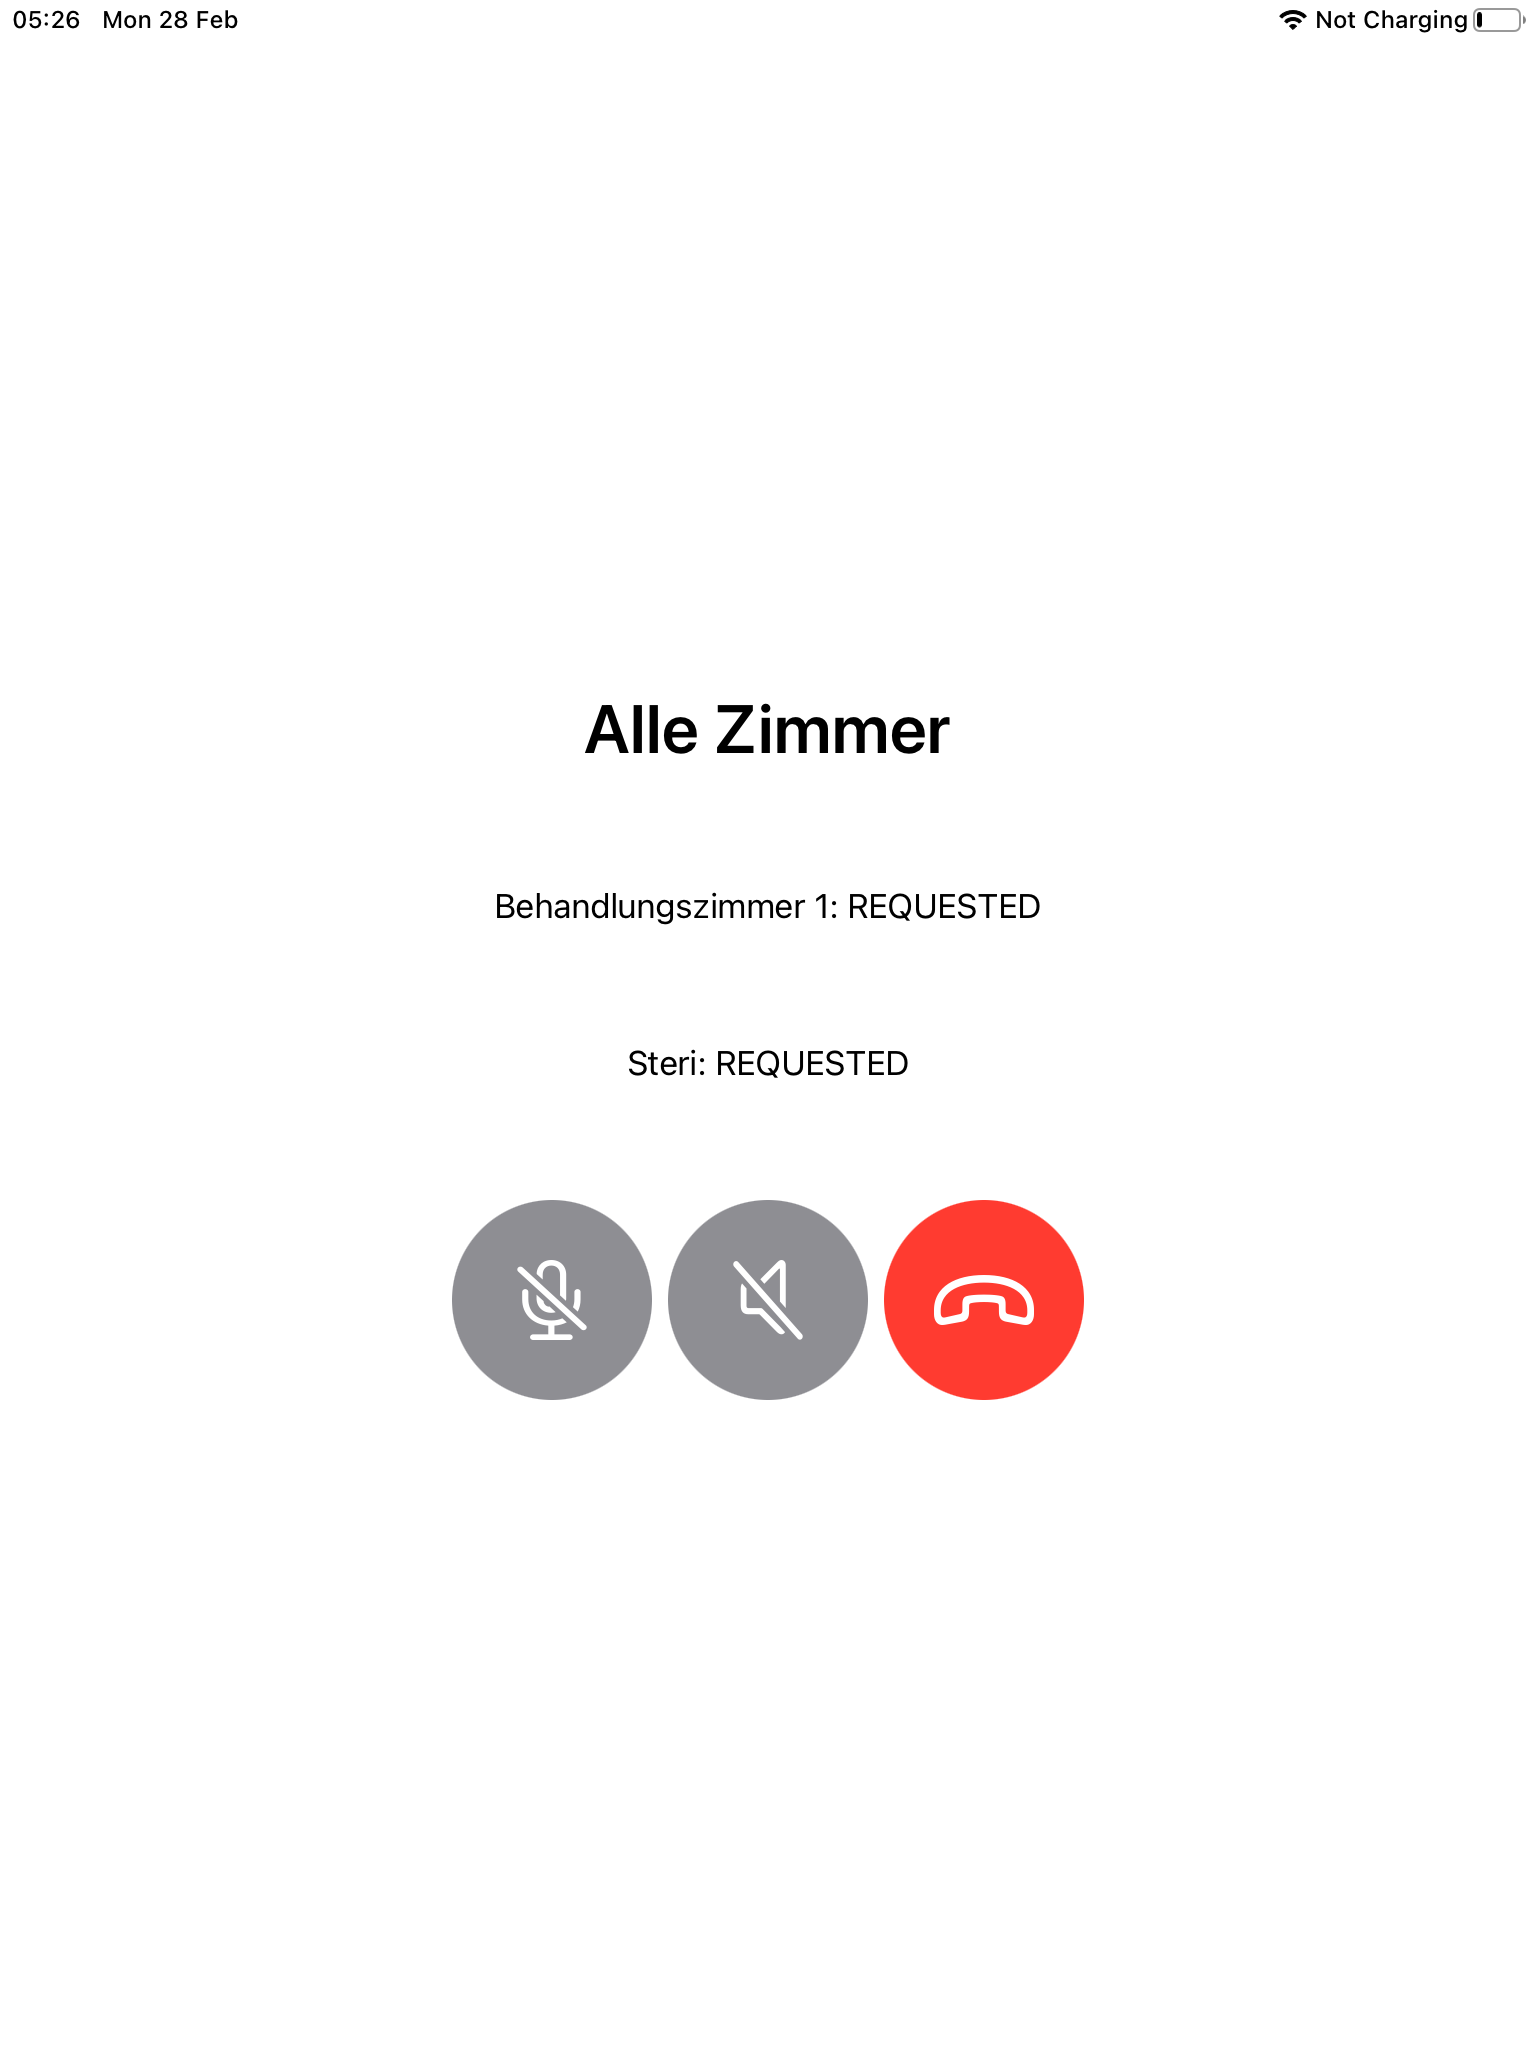
\includegraphics[width=\textwidth]{graphics/screenshots/app/call}}
        \caption{Aktiver Anruf}
    \end{minipage}
    \label{fig:MobileClient-ScreensIntroduction}
\end{figure}

Auf der Startseite der Applikation können per Knopfdruck Benachrichtigungen versendet und Sprachverbindungen gestartet werden.
Empfangene Benachrichtigungen werden als Push-Benachrichtigung angezeigt und in einer Inbox gesammelt.
Bei entsprechender Konfiguration wird zudem der Inhalt von empfangenen Benachrichtigungen automatisch vorgelesen.
Sprachverbindungen können zwischen zwei oder mehr Teilnehmern aufgebaut werden.
Das System unterstützt sowohl private Gespräche als 1:1 Verbindungen wie auch Gruppenunterhaltungen als 1:N Verbindungen.

Welche Buttons und damit welche Benachrichtigungen und Sprachverbindungen zur Verfügung stehen, wird durch Praxisadministratoren konfiguriert.
Die Konfiguration von Buttons für Sprachverbindungen beinhaltet, mit welchen Empfängern eine Verbindung aufgebaut wird.
Die Konfiguration von Buttons für Benachrichtigungen definiert den Inhalt der Benachrichtigung, welche Empfänger sie erhalten und ob die Benachrichtigung vorgelesen wird.
Für die Verwaltung dieser Konfiguration kann durch eine Weboberfläche vorgenommen werden.
Abbildung 1.3 zeigt die Übersicht verfügbarer Benachrichtigung in dieser Weboberfläche.

\begin{figure}[h]
    \centering
    \begin{minipage}[b]{1\textwidth}
        \fbox{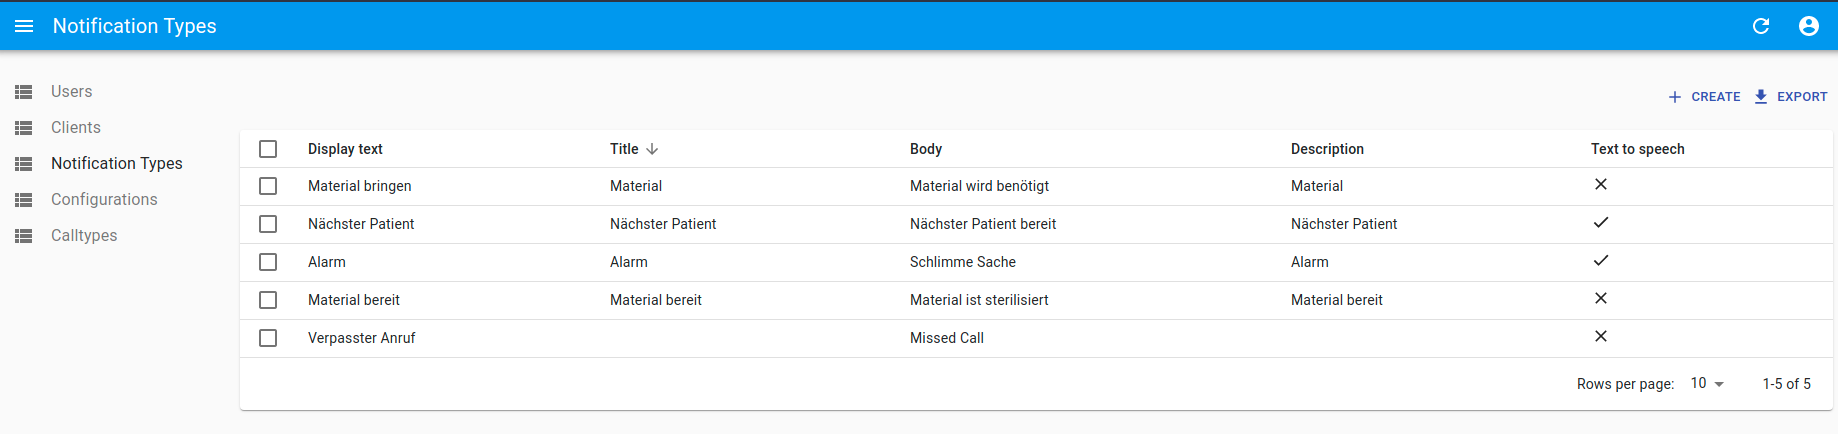
\includegraphics[width=\textwidth]{graphics/screenshots/admin_ui_notification_types}}
        \caption{Praxisruf Startseite}
    \end{minipage}
    \label{fig:AdminUI-Introduction}
\end{figure}

Die Grundlage für das entwickelte Praxisrufsystem wurde im Rahmen der Projektarbeit ''IP5 Cloudbasiertes Praxisrufsystem'' erarbeitet.
Im Rahmen des Vorgängerprojektes wurde bereits ein Praxisrufsystem mit eingeschränktem Funktionsunmfang entwickelt.
Die in diesem Projekt entwickelte Lösung ist eine Erweiterung des bestehenden Systems.
Das zuvor umgesetzte System unterstützt das Versenden und Empfangen von Benachrichtigungen.
Sprachsynthese für Benachrichtigungen und Sprachverbindungen für eine Gegensprechanlage konnten im Rahmen des Vorgängerprojektes nicht umgesetzt werden.
Die zentrale Aufgabenstellung für dieses Projekt war es, das System zu erweitern so, dass Benachrichtigungen vorgelesen und Sprachverbindungen aufgebaut werden können.
Die Bedienung des Praxisrufsystems soll weiterhin über eine mobile Applikation möglich sein.
Dazu soll eine neue, native iOS Applikation entwickelt werden.
Diese ersetzt die bestehende App und muss alle bestehenden Funktionen unterstützten.
Sie muss zudem Sprachverbindungen zu anderen Teilnehmern aufbauen und den Inhalt von Benachrichtigungen vorlesen können.

Wie in der Aufgabenstellung beschrieben, hat eine Marktanalyse im Vorfeld dieses Projektes gezeigt, dass bestehende kommerzielle Praxisrufsysteme veraltete Technologien einsetzten.
Diese Systeme sind aufwändig zu installieren und skalieren schlecht.
Sie können weiter nicht einfach in ein TCP/IP-Netzwerk eingebunden und über externe APIs angesteuert werden.\cite{aufgabenstellung}
Das im Rahmen des Vorgängerprojektes umgesetzte System löst diese Probleme bereits teilweise.
Mit dem Cloudservice bietet das System einen zentralen Dienst, welcher über eine Http Schnittstelle ansprechbar ist.
Diese ermöglicht die Verwaltung der Systemkonfiguration und stellt Benachrichtigung anhand der Konfiguration an relevante Empfänger zu.
Dadurch ist es einfacher möglich, das System in Netzwerke einzubinden, zu skalieren und neue Endgeräte anzubinden.
Das Vorgängersystem unterstützt aber noch nicht alle Funktionen, die ein Praxisrufsystem bieten muss.
Die meisten kommerziell erhältlichen Lösungen können als Gegensprechanlage verwendet werden\cite{aufgabenstellung}.
Ein vollständiges Praxisrufsystem muss deshalb unbedingt als Gegensprechanlage verwendet werden können.
Mit der Integration von Sprachsynthese für Benachrichtigungen kann sich das System weiter von bestehenden Lösungen absetzten.
Ein weiterer Schwachpunkt des Vorgängerprojektes ist die mobile Applikation.
Diese wurde mit einer geteilten Codebasis für iOS und Android entwickelt.
Im Fazit des Vorgängerprojekts wurde festgehalten, dass diese Applikation idealerweise neu als native Applikation entwickelt werden sollte.
Dadurch könne effizienter Betrieb, Wartung sowie Hardware- und Betriebssystemkomaptibilität langfristig gewährleistet werden.\cite{ip5}

Das umgesetzte System besteht aus drei Applikationen.
Der zentrale Cloudservice dient zur Verwaltung der Konfiguration und dem Vermitteln von Nachrichten zwischen Endgeräten.
Das Admin UI bietet eine Weboberfläche mit der die Konfiguration des Cloudservice verwaltet werden kann.
Mit dem Mobile Client bietet das System eine iOS App über welche Sprachverbindungen aufgebaut und Benachrichtigungen versendet werden können.
Für das Versenden von Benachrichtigungen, sendet ein Mobile Client eine HTTP Anfrage an den Cloudservice.
Der Cloudservice findet in der Konfiguration alle relevanten empfänger und leitet die Benachrichtigung an diese weiter.
Für die Zustellung von aus dem Cloudservice an Mobile Clients wird Firebase Cloud Messaging verwendet.

Für die Synthese von Sprachdaten wurde eine Anbindung an AWS Polly im Cloudservice implementiert.
Der Cloudservice bietet neue eine Http Schnittstelle, über welche Clients Sprachdaten für Benachrichtigungen beziehen können.
Durch diese Lösung müssen die Endgeräte die Anbindung an den Sprachsyntheseprovider nicht selbst implementierten.
Dies bietet den Vorteil das der Provider leicht ausgewechselt werden kann und dass die Anbindung von zukünftige Platformen übernommen werden kann.

\begin{figure}[h]
    \centering
    \begin{minipage}[b]{0.75\textwidth}
        \fbox{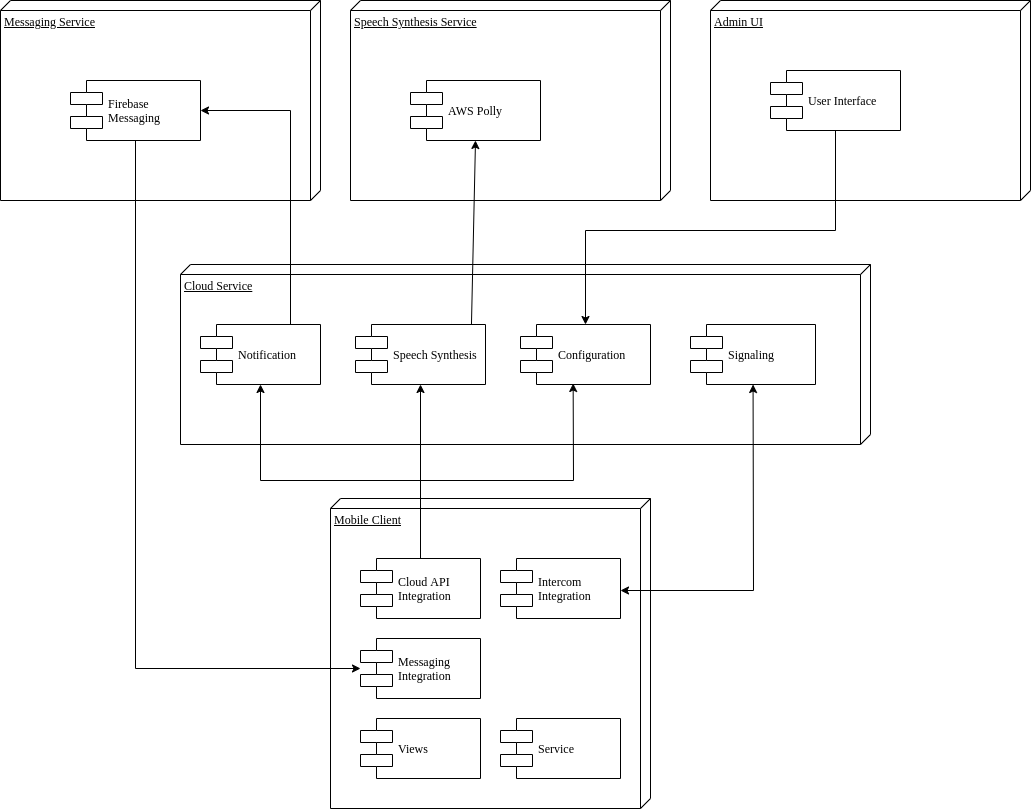
\includegraphics[width=\textwidth]{graphics/diagramms/Component_System_V02}}
        \caption{Systemarchitektur Praxisruf}
    \end{minipage}
\end{figure}

Sprachverbindungen zwischen Mobile Clients werden als Peer To Peer Verbindungen aufgebaut.
Diese Verbindungen wurden mit der Technologie WebRTC umgesetzt.
WebRTC steht für Web Real-Time Communication.
Dabei handelt es sich um ein Open Source Projekt, welches Echtzeitkommunikation für mobile Applikationen und Browser Applikationen ermöglicht.
Damit Peer To Peer Verbindungen zwischen Mobile Clients aufgebaut werden können, müssen diese Meldungen austauschen können.
Um dies zu ermöglichen, wurde der Cloudservice um ein Modul ''Signaling'' erweitert.
Dieses Modul bietet eine Websocketschnittstelle, über welche die nötigen Signalmeldungen ausgetauscht werden können.
Jeder Mobile Client der für Sprachverbindungen verfügbar ist, baut bei der Anmeldung eine Websocketverbindung zum Signaling Modul auf.
Über diese Verbindung sendet und empfängt er alle Signalmeldungen, die für den Verbindungsaufbau notwendig sind.

Im folgenden Bericht werden die erarbeiteten Konzepte und Resultate vorgestellt.
Zunächst werden Vorgehensweise, Projektplan und die Organisation des Projekts vorgestellt.
Anschliessend werden die Anforderungen, welche zu Beginn des Projekts definiert wurden, beschrieben.
Es folgt eine Technologie Evaluation für Sprachsynthese und Gegensprechanlage.
Dabei werden mögliche Optionen beschrieben und anschliessend eine begründete Entscheidung beschrieben.
Das darauffolgende Kapitel beschreibt das detaillierte technische Konzept für Funktionsweise und Architektur des Systems.
Es wird beschrieben, wie die Funktionen Gegensprechanlage und Sprachsynthese umgesetzt wurden.
Dabei wird insbesondere darauf eingegangen, wie die bestehende und neue Funktionen im neuen nativen Mobile Client integriert werden.
Weiter werden die notwendigen Abläufe, Kommunikationskanäle und Datenmodelle beschrieben.
Nach dem Konzept werden die Resultate zusammengefasst und die umgesetzten Ansichten des nativen iOS App abgebildet.
Am Ende der Arbeit stehen ein Fazit und Schlusswort mit Empfehlungen für das weitere Vorgehen.

\clearpage

    \section{Vorgehensweise}

\subsection*{Project Plan}

Lorem Ipsum

\subsection*{Meilensteine}

Lorem Ipsum

\clearpage

    \section{Anforderungen}\label{sec:anforderungen}

Es gibt drei Rollen von Stakeholdern, welche Anforderungen an Praxisruf stellen.
Die meisten Benutzer des Systems fallen in die Rolle Praxismitarbeitende.
Diese verwenden die mobile Applikation von Praxisruf, um in der Praxis miteinander zu kommunizieren.
Neben der Rolle der Praxismitarbeitenden, arbeitet auch die Rolle des Praxisverantwortlichen mit dem Praxisrufsystem.
Diese Benutzergruppe ist dafür verantwortlich, Praxisruf für Praxismitarbeitende zu konfigurieren.
Als dritte Rolle hat zudem der Auftraggeber ein Interesse daran, dass gewisse Rahmenbedingungen gesetzt und eingehalten werden.{Siehe Projektbericht Cloudbasiertes Praxisrufsystem \cite{ip5}}. \\

Im folgenden Kapitel werden die Anforderungen dokumentiert, die bei Projektstart ermittelt wurden.
Die Anforderungen werden dabei aus fachlicher Sicht mit User Stories festgehalten.
Jede User Story beschreibt ein konkretes Bedürniss einer Stakeholdergruppe.

\subsection*{User Stories}

\subsubsection*{Praxismitarbeitende}

\begin{table}[h]
    \centering
    \begin{tabular}{|l|p{15cm}|}
        \hline
        \textbf{Id} & \textbf{Anforderung}                                                                                                                                                                                      \\
        \hline
        U01           & Als Praxismitarbeiter/in möchte ich alle Funktionen aus der existierenden Applikation weiterhin verwenden können, damit mir diese weiterhin die Arbeit erleichtern. \footnote[2]{}                        \\
        \hline

        U02           & Als Praxismitarbeiter/in möchte ich, dass wichtige eingehende Benachrichtigungen vorgelesen werden, damit den Inhalt der Benachrichtigung kenne, ohne meine Aufmerksamkeit auf den Bildschirm zu richten. \\
        \hline
        U03           & Als Praxismitarbeiter/in möchte ich, das Vorlesen von Benachrichtigungen deaktivieren können, damit ich bei der Arbeit nicht unnötig gestört werde.                                                       \\
        \hline
        U04           & Als Praxismitarbeiter/in möchte ich, per Button eine Sprachverbindung zu einem anderen Praxiszimmer aufbauen können, damit ich mich mit einer anderen Person absprechen kann.                             \\
        \hline
        U05           & Als Praxismitarbeiter/in möchte ich, per Button eine Sprachverbindung zu mehreren anderen Praxiszimmern aufbauen können damit, ich mich mit mehreren anderen Personen absprechen kann.                    \\
        \hline
        U06           & Als Praxismitarbeiter/in möchte ich über geöffnete Sprachverbindungen in Echtzeit kommunizieren können damit es die Funktion einer Gegensprechanlage wirklich erfüllt.                                    \\
        \hline
        U07           & Als Praxismitarbeiter/in möchte ich nur Buttons für Sprachverbindungen sehen, die für mich relevant sind.                                                                                                 \\
        \hline
        U08           & Als Praxismitarbeiter/in möchte ich benachrichtigt werden, wenn ein anderes Zimmer eine Sprachverbindung öffnet, damit ich auf die Anfrage Antworten kann.                                                \\
        \hline
        U09           & Als Praxismitarbeiter/in möchte ich vergangene und verpasste Sprachverbindungen nachvollziehen können, damit ich mich zurückmelden kann.                                                                  \\
        \hline
        U10           & Als Praxismitarbeiter/in möchte ich, dass eingehende Sprachverbindungen aus anderen Praxiszimmern automatisch geöffnet werden damit ich meine Hände für besseres brauchen kann.                           \\
        \hline
        U11           & Als Praxismitarbeiter/in möchte ich, direkte Sprachverbindungen aus anderen Praxiszimmern trennen können damit ich ein Gespräch beenden kann.                                                             \\
        \hline
        U12           & Als Praxismitarbeiter/in möchte ich, aus Sprachverbindungen zu mehreren Praxiszimmern (Gruppenunterhaltungen) austreten können, damit ich nicht unnötig bei der Arbeit gestört werde.                     \\
        \hline
    \end{tabular}\label{tab:userstories1}
\end{table}

\clearpage

\subsubsection*{Praxisadministrator}

\begin{table}[h]
    \centering
    \begin{tabular}{|l|p{15cm}|}
        \hline
        \textbf{Id} & \textbf{Anforderung}                                                                                                                                                                                                    \\
        \hline
        U13           & Als Praxisadministrator möchte ich konfigurieren können, welche Benachrichtigungen dem Praxismitarbeitenden vorgelesen werden, damit nur relevante Benachrichtigungen vorgelesen werden.                                \\
        \hline
        U14           & Als Praxisadministrator möchte ich konfigurieren können, aus welchen Zimmern Sprachverbindungen zu welchen anderen Zimmern aufgebaut werden können, damit die Mitarbeitendend das System effizient bedienen können.     \\
        \hline
        U15           & Als Praxisadministrator möchte ich Benachrichtigungen, Clients und Benutzer wie zuvor konfigurieren können, damit ich das System weiterhin auf meine Praxis zuschneiden und bestehende Konfigurationen übernehmen kann. \\
        \hline
    \end{tabular}\label{tab:userstories2}
\end{table}

\subsubsection*{Auftraggeber}

\begin{table}[h]
    \centering
    \begin{tabular}{|l|p{15cm}|}
        \hline
        \textbf{Id} & \textbf{Anforderung}                                                                                                                                                             \\
        \hline
        U16           & Als Auftraggeber möchte ich die bestehende Betriebsinfrastruktur übernehmen, um von der bereits geleisteten Arbeit profitieren zu können.                                        \\
        \hline
        U17           & Als Auftraggeber möchte ich, dass die bestehende Komponenten des Systems wo immer möglich weiter verwendet werden, um von der bereits geleisteten Arbeit profitieren zu können. \\
        \hline
        U18           & Als Auftraggeber möchte ich, der bestehende Mobile Client als native iOS Applikation ungeschrieben wird, um Wartbarkeit und Gerätekompatibilität zu gewährleisten. \\
        \hline
    \end{tabular}\label{tab:userstories3}
\end{table}

\subsection*{Features}

Aus den User Stories ergeben sich drei Features, welche mit dem Projekt "P2P Sprachübertragung in Praxisrufsystemen" umgesetzt werden müssen.

\begin{table}[h]
    \centering
    \begin{tabular}{|l|p{15cm}|}
        \hline
        \textbf{Id} & \textbf{Feature}                                                                                                                                                             \\
        \hline
        F01           & Migration des bestehenden Mobile Client                                        \\
        \hline
        F02           & Text To Speech \\
        \hline
        F03           & Gegensprechanlage \\
        \hline
    \end{tabular}\label{tab:features}
\end{table}

Diese Features dienen zur Aufteilung der Umsetzungsphase.
F01 Migration des bestehenden Mobile Client bildet die Grundalge für die anderen Features und wird deshalb als erstes Umgesetzt.
F02 Text To Speech ist eng mit der bestehenden Funktionalität verbunden.
Es soll deshalb möglichst zeitnah nach F01 umgesetzt werden.
F03 Gegensprechanlage ist das Kernstück der neuen Funktionalität.
Dieses Feature kann erst umgesetzt werden, wenn die Grundlagenarbeit von F01 umgesetzt ist.


\clearpage

    \section{Technologie Evaluation}

Hier werden die Technologien und Frameworks mit denen das Projekt umgesetzt wird evaluiert.


\subsection{Appentwicklung IOS}

Mit dem Projekt ''IP5 Cloudbasiertes Praxisrufsystem''\cite{ip5} wurde bereits eine mobile Applikation für Praxisruf umgesetzt.
Mit dieser Applikation können bereits heute Benachrichtungen über Praxisruf versendet und empfangen werden.
Die bestehende Applikation wurde mit Nativescript als Multi-Platform Applikation gebaut.
Um die Wartbarkeit und Hardware- sowie Betriebssystemkomaptibilität zu gewährleisten wurde im Fazit des Vorgängerprojekts empfohlen,
die Applikation neu als native Applikation für iOS und Android zu schreiben.\cite{ip5}

Mit diesem Projekt soll die Applikation dementsprechend neu als native iOS Applikation umgesetzt werden.
Dabei ist es wichtig, dass sämtliche bestehende Funktionalität auch im neu entwickelten nativen Mobile Client zur Verfügung steht.
Um weiterhin Benachrichtungen senden und empfangen zu können, muss die gewählte Technologie es ermöglichen Firebase Cloud Messaging anzubinden
und Push Benachrichtigungen im Vorder- sowie im Hintergrund empfängen können.
Weiter muss die Technologie es ermöglichen, Hintergrundtasks zu erstellen und Audiosignale abzuspielen.
Dadurch wird es möglich, regelmässig ein Signal abzuspielen um die Praxismitarbeitenden an verpasste Benachrichtigungen zu erinnern.

\subsubsection*{Programmiersprache}

Für die Entwicklung von nativen iOS Applikationen ist die Programmiersprache Swift als Standard gesetzt.\cite{ios_swift}


\subsubsection*{Framework}

Für die Umsetzung von iOS Applikationen stellt Apple die zwei Frameworks UIKit\cite{ios_uikit} und SwiftUI\cite{ios_swift_ui} zur Verfügung.
UIKit ist das ältere der beiden Frameworks und ist seit iOS 2.0 verfügbar.
Dementsprechend ist das Framework ausgereifter und bietet viele Funktionen zur Integration einer Applikation mit iOS.
Es hat allerdings den Nachteil das es schwerer zu erlernen und langsamer zu schreiben ist. (Citation Needed)

SwiftUI ist deutlich neuer als UIKit und steht seit iOS 13.0 zur Verfügung.
Es hat eine tiefere Einstiegshürde als UIKit und ist grundsätzlich einfacher zu schreiben und warten (Citation Needed).
In den Worten von Apple selbst: "SwiftUI helps you build great-looking apps across all Apple platforms with the power of Swift — and as little code as possible."\cite{ios_swift_ui}

SwiftUI bietet zudem ausgezeichnete Integration des Entwicklungsworkflows in die XCode Entwicklungsumgebung.
Es bietet schnelle live previews der Komponenten die geschrieben werden.
Dies vereinfacht Design und Umsetzung der Ansichten.

SwiftUI bietet weiter viele Standardkomponenten wie Listenansichten, Formfelder und andere UIKomponenten, die es einfacher machen
eine Benutzeroberfläche zu erstellen die den Look und Feel einer nativen iOS Applikation hat.
Die Ansichten aus dem bestehenden Mobile Client können mit SwiftUI umgesetzt werden.





Alles nötige unterstützt.
Neuer und encouraged.


\subsection*{Unterstützung Features}

Firebase Messaging mit App Delegate \cite{firebase_ios}

Erinnerungen mit Timer\cite{ios_timer} und BGTaskScheduler\cite{ios_bgtaskscheduler}


Optionen \\

Swift ist standard \\
UIKit oder SwiftUI \\

SwiftUI ist neu und die Richtung in die Apple seit einiger Zeit pushed. \\
Es wird SwiftUI genommen, weil es der neue Standard ist. \\
Gewisse Hooks in den IOS Lifecycle sind mit rein SwiftUI noch nicht möglich. \\
Die entsprechenden Teil (AppDelegates) können auch in SwiftUI verwendet werden. \\

Kleiner POC wurde mit SwiftUI erstellt um zu verifizieren, dass Anforderungen von oben möglich sind. \\

\subsubsection*{Zusammenfassung}

Entscheidung: \\

Target IOS15 \\
Swift 5 \\
SwiftUI 3.0 \\

\clearpage


\subsection{Text To Speech}

Lorem Ipsum

\clearpage


\subsubsection{VOIP Kommunikation}

Lorem Ipsum

\clearpage


    \section{Konzept}

Lorem ipsum

\subsection{Migration Benachrichtigungen}

Mit IP5 wurde bereits ein Client umgesetzt.
Dieser muss für IP6 migiert werden.

Architektur Anbindung Rest \\
Architektur Anbindung Firebase \\

\clearpage


\subsection{Integration Text To Speech}

\subsubsection*{Benutzeroberfläche}

Erweiterung Inbox um T2S Icon. \\
Erweiterung Admin UI um Checkbox. \\
Zusätzlich Configuration Page mit preferences. \\

\subsubsection*{Konfiguration}
Erweiterung NotificationType um ein boolean Flag für isTextToSpeech.
Wenn Aktiviert, wird Benachrichtigung bei Empfang vorgelesen.
Text To Speech kann auf Client Seite dekativiert werden.
Ist es deaktiviert, werden keine Benachrichtigungen vorgelesen.
Audio Signal, dass Benachrichtung empfangen wurde ertönt aber trotzdem.
Keine zusätzlichen Endpoints am Cloud Service nötig. \\


\subsection*{Laufzeitsicht}

Empfang und Versenden gleich wie bei IP5.
Benachrichtigung enthält zudem neu Flag ob T2S gebraucht werden soll.
Wenn ja, wird Vorlesen an T2S Service delegiert.

\begin{figure}[h]
    \centering
    \begin{minipage}[b]{0.9\textwidth}
        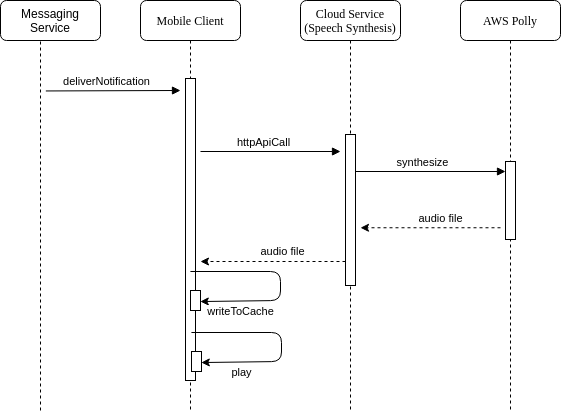
\includegraphics[width=\textwidth]{graphics/diagramms/Sequence_Speech_Synth_V01}
        \caption{Ablauf Benachrichtigung empfangen}
    \end{minipage}
\end{figure}

\clearpage

\subsection{Integration Gegensprechanlage}

\subsubsection*{Benutzeroberfläche}

Button Screen wie IP5 \\
Active Call Screen \\
Erweiterte Inbox \\
Neue Screens für Gegensprechanlage. \\
Erweiterung Admin UI für Konfiguration CallType \\


\subsubsection*{Konfiguration}
Erweiterung Configuration Domain um CallType.
Hat text property, dass als Anzeige auf dem Button dient.
Hat Liste von Clients, die im Call angesprochen werden können.

\subsubsection*{Laufzeitsicht}

\begin{figure}[h]
    \centering
    \begin{minipage}[b]{0.9\textwidth}
        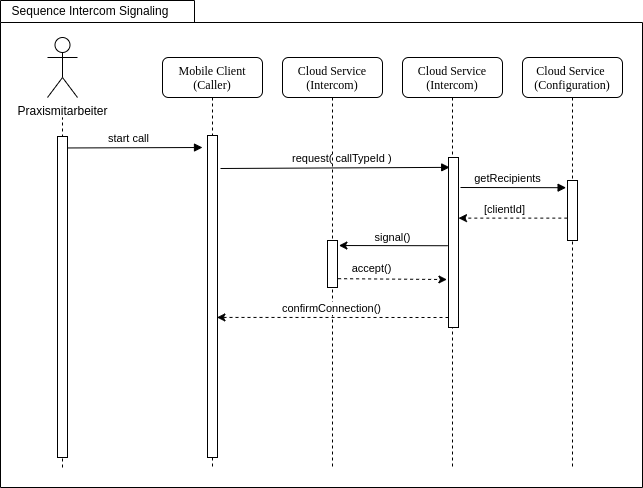
\includegraphics[width=\textwidth]{graphics/diagramms/Sequence_Intercom_Broking_V01}
        \caption{Ablauf Verbindungsaufbau Gegensprechanalge}
    \end{minipage}
\end{figure}

\clearpage

\subsection{Übersicht Erweiterung Praxisruf Cloud Service}

<< Erweitertes ERD für Configuration Domain (Cloud Service) >>

\clearpage

    
\section{Umsetzung}

Lorem ipsum
\clearpage

    \section{Schluss}

Lorem Ipsum

\clearpage



%%---APPENDIX----------------------------------------------------------------------------
    \renewcommand\refname{Literaturverzeichnis}
\addcontentsline{toc}{section}{Literaturverzeichnis}
\printbibliography
\cleardoublepage
\listoffigures

\appendix
\clearpage
\section{Aufgabenstellung}\label{sec:aufgabenstellung}
\begin{figure}[h]
    \centering
    \begin{minipage}[b]{0.8\textwidth}
        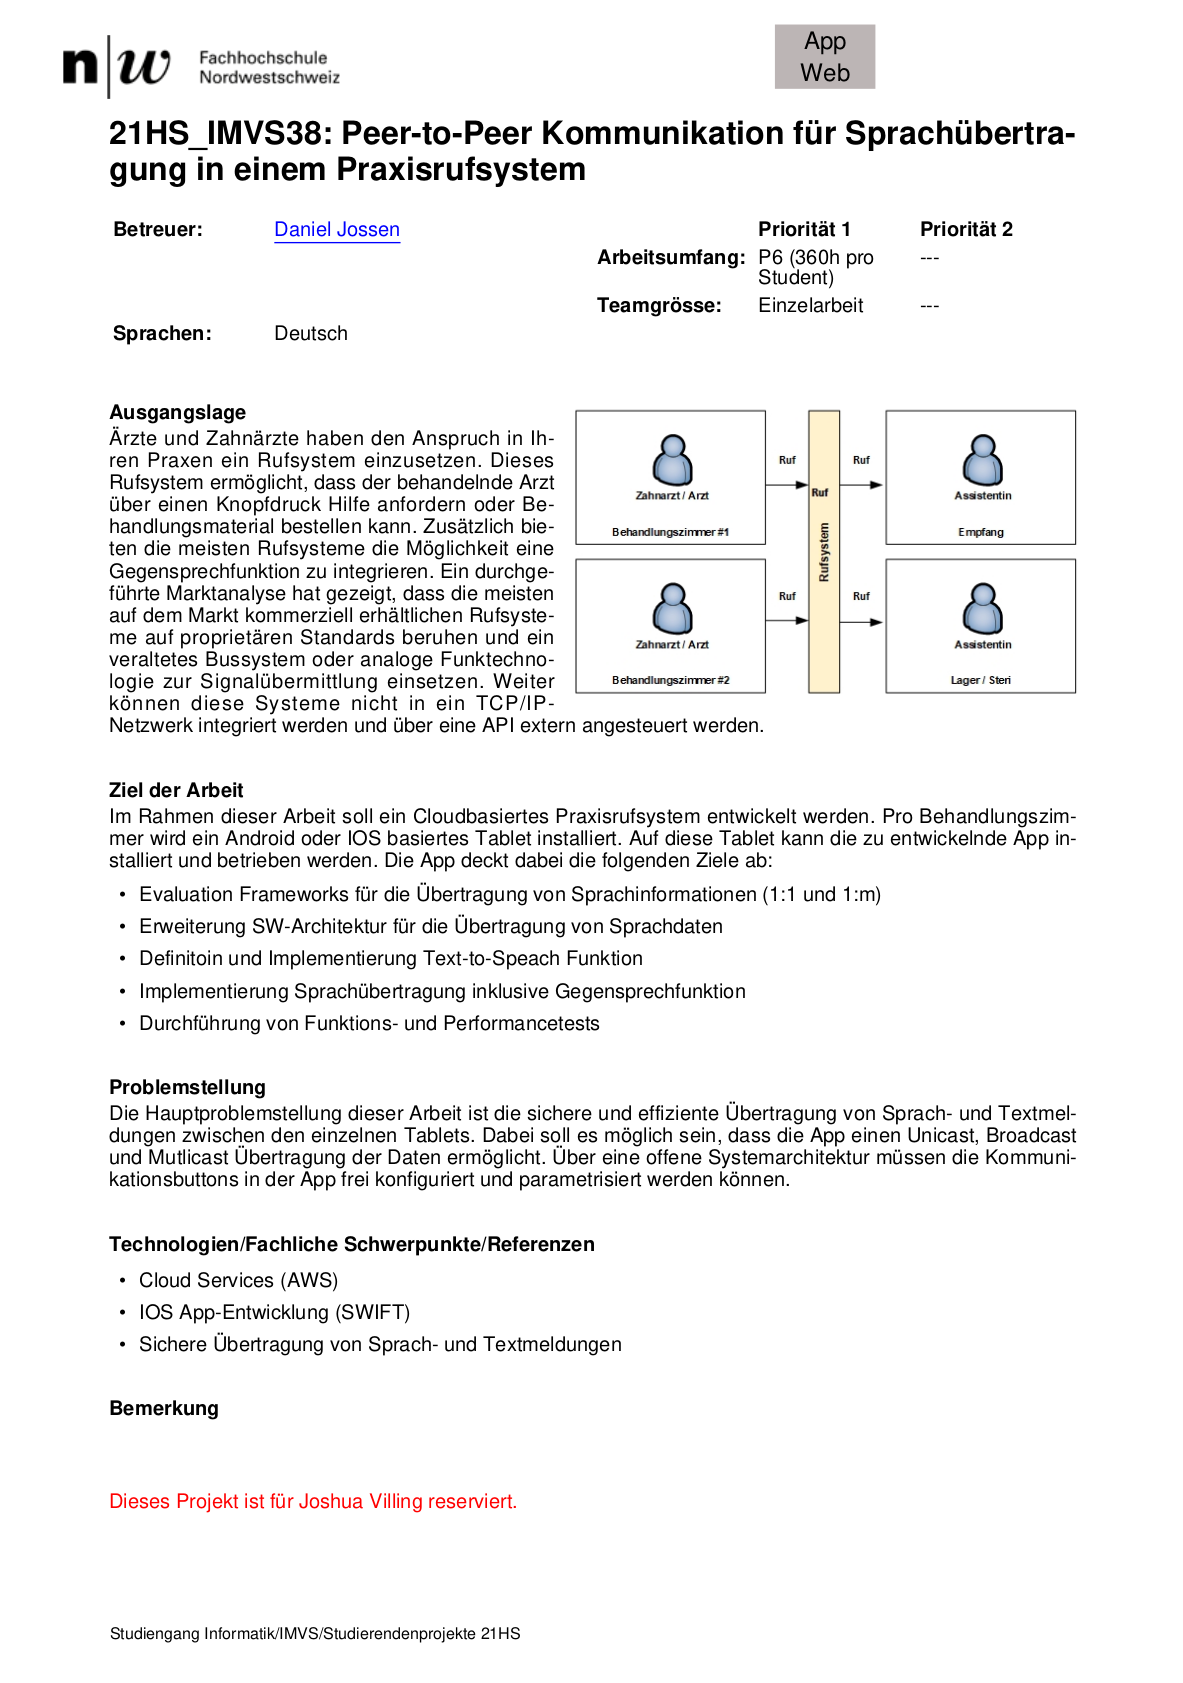
\includegraphics[width=\textwidth]{graphics/aufgabenstellung}
        \caption{Aufgabenstellung}
    \end{minipage}\label{fig:aufgabenstellung}
\end{figure}

\clearpage

\section{Quellcode}\label{sec:quellcode}

Sämtlicher Quellcode der im Rahmen des Projektes entsteht, wurde mit Git verwaltet. Der Quellcode ist für Berechtigte unter github.com einsehbar\footnote{\url{https://github.com/users/jsvilling/projects/3}}.
Berechtigungen können bei Joshua Villing angefordert werden.

\clearpage

\section{Ehrlichkeitserklärung}

«Hiermit erkläre ich, die vorliegende Projektarbeit IP6 - Cloudbasiertes Praxisrufsystem selbständig und nur unter Benutzung der angegebenen Quellen verfasst zu haben.
Die wörtlich oder inhaltlich aus den aufgeführten Quellen entnommenen Stellen sind in der Arbeit als Zitat bzw. Paraphrase kenntlich gemacht.
Diese Projektarbeit ist noch nicht veröffentlicht worden.
Sie ist somit weder anderen Interessierten zugänglich gemacht noch einer anderen Prüfungsbehörde vorgelegt worden.»

\begin{tabbing}
    \\
    \\
    \\
    Left \= Middle \=  \= Right \kill
    Name \> \> \>    Joshua Villing\\
    Ort \> \> \>    Aarau \\
    Datum \> \> \>    01.03.2022\\
    \\
    Unterschrift \> \> \>     ............................\\

\end{tabbing}




\end{document}
